%%%%%%%%%%%%%%%%%%%%%%%%%%%%%%%%%%%%%%%%%%%%%%%%
%%%%%%%%%%%%%%%%%%%%%%%%%%%%%%%%%%%%%%%%%%%%%%%%
%
%		Kommentar
%		Ein nettes old school template.......
%		last modified: 27/03/07
%
%%%%%%%%%%%%%%%%%%%%%%%%%%%%%%%%%%%%%%%%%%%%%%%%
%%%%%%%%%%%%%%%%%%%%%%%%%%%%%%%%%%%%%%%%%%%%%%%%
\documentclass[a4book,11pt,twoside]{scrbook}
\usepackage{eurosym}
\usepackage[german]{babel}
\usepackage{amsmath}
\usepackage{amssymb}
\usepackage[automark]{scrpage2}	%Kopfzeile Autoinhalt (Kapitel)
\usepackage{graphics}
\usepackage{color}
\usepackage{graphicx}
\usepackage{longtable}
\usepackage{lscape}
\usepackage{hhline}
\usepackage{booktabs}
\usepackage{IFSlogo}
% \usepackage[T1]{fontenc}
% \usepackage[pdftex]{hyperref}
\usepackage{makeidx}
\selectlanguage{german}
\setlength{\parindent}{0pt}  % setzt sie Einrückung nach einem Umbruch zurück

%%%%%%%%%%%%%%%%%%%%%%%%%%%%%%%%%%%%%%%%%%%%%%%%
%		Sachregister-Erstellung
%		Begriffe werden mit Befehl \index{} aufgenommen
% 		Index erstellen in Konsole makeindex -g -s style.ist Vorlage.idx 
%%%%%%%%%%%%%%%%%%%%%%%%%%%%%%%%%%%%%%%%%%%%%%%% 
\makeindex


%%%%%%%%%%%%%%%%%%%%%%%%%%%%%%%%%%%%%%%%%%%%%%%%
%		ETH-Schrift einführen
%%%%%%%%%%%%%%%%%%%%%%%%%%%%%%%%%%%%%%%%%%%%%%%% 

\usepackage[standard-baselineskips]{cmbright} % Mathematikschrift die in etwa ETH-Light entspr.
\renewcommand{\sectfont}{\bfseries}

%\renewcommand{\familydefault}{let} 
%\renewcommand{\seriesdefault}{let}
%\renewcommand{\shapedefault}{let}
%\renewcommand{\sfdefault}{let}
\renewcommand{\rmdefault}{let}


% \DeclareFixedFont{\x}{T1}{let}{m}{n}{10}
% \DeclareFixedFont{\xb}{T1}{let}{m}{n}{10}
% \newfont{\xiiiv}{letr8t at 8.0pt}
% \newfont{\xiiivb}{letb8t at 8.0pt}


%%%%%%%%%%%%%%%%%%%%%%%%
% Schriftengefrickel
%%%%%%%%%%%%%%%%%%%%%%%%%
\usepackage{fontspec}
\usepackage{sectsty}

\partfont{\font \x="DINNeuzeitGroteskStd-Light" at 40pt\x}
\chapterfont{\font \x="DINNeuzeitGroteskStd-Light" at 32pt\x}
\sectionfont{\font \x="DINNeuzeitGroteskStd-Light" at 16pt\x}
\subsectionfont{\font \x="DINNeuzeitGroteskStd-Light" at 14pt\x}
\subsubsectionfont{\font \x="DINNeuzeitGroteskStd-Light" at 14pt\x}
\paragraphfont{\font \x="DINNeuzeitGroteskStd-Light" at 14pt\x}
\newfontface\swashed[Contextuals=Swash, Ligatures=Common]{Adobe Garamond Pro Italic}
\newfontface\foo[Numbers={OldStyle},Contextuals=Swash, Ligatures=Common]{Adobe Garamond Pro}
\newfontface\foofat[Numbers={OldStyle},Contextuals=Swash, Ligatures=Common]{Adobe Garamond Pro Bold}


\usepackage[a4paper,left=4.0cm, right=4.0cm,top=3.0cm, bottom=3.0cm]{geometry}
	
%%%%%%%%%%%%%%%%%%%%%%%%%%%%%%%%%%%%%%%%%%%%%%%%
%		eigenen Stil definieren
%%%%%%%%%%%%%%%%%%%%%%%%%%%%%%%%%%%%%%%%%%%%%%%% 
\pagestyle{scrheadings}
\renewcommand*{\chapterpagestyle}{scrheadings} 
\clearscrheadfoot 
\ihead{\textsf{\headmark}} 
\ohead{\pagemark}
\setheadsepline{.4pt}
\setfootsepline{.4pt}
\ifoot{}
\ofoot{\footnotesize{\textsc{Hsr, Silvio Heuberger}}}


% frickelabst�nde

% abst�nde und sooooo
\setlength{\columnsep}{10mm}
\setlength{\parskip}{2.5mm}

%two column float page must be 90% full
\renewcommand\dblfloatpagefraction{.90}
%two column top float can cover up to 80% of page
\renewcommand\dbltopfraction{.80}
%float page must be 90% full
\renewcommand\floatpagefraction{.90}
%top float can cover up to 80% of page
\renewcommand\topfraction{.80}
%bottom float can cover up to 80% of page
\renewcommand\bottomfraction{.80}
%at least 10% of a normal page must contain text
\renewcommand\textfraction{.1}


%%%%%%%%%%%%%%%%%%%%%%%%%%
% listings for everyone

\definecolor{defgray}{cmyk}{0.3,0.05,0,0.43}
\usepackage[plainpages={false}, bookmarks, pdfstartview={FitV}, colorlinks, linkcolor=defgray]{hyperref}


\usepackage{listings}
\lstset{% general command to set parameter(s)
basicstyle=\ttfamily\small, % print whole listing small
%basicstyle=\small,
commentstyle=\color{defgray}, % comments
stringstyle=\ttfamily, % typewriter type for strings
showstringspaces=false,
keywordstyle=\bfseries\color{blue},
numbers=left,
numberstyle=\color{defgray}\tiny,
frame=single,
%frame=shadowbox,
%frameround=tttt,
rulesepcolor=\color{defgray},
language={ruby}
} % no special string spaces


% make monospace font the same size (optocally) as Arno Pro
\setmonofont[Scale=0.9]{ITC American Typewriter Std Condensed}
\defaultfontfeatures{Scale=MatchLowercase,Mapping=tex-text}


\begin{document}
\renewcommand{\theequation}{\thesection.\arabic}
\addtokomafont{caption}{\small}
\setkomafont{captionlabel}{\sffamily\bfseries}
\numberwithin{equation}{section}
\pagenumbering{Roman}
\setcapindent*{1em}

%%%%%%%%%%%%%%%%%%%%%%%%%%%%%%%%%%%%%%%%%%%%%%%%
%		Titelseite
%%%%%%%%%%%%%%%%%%%%%%%%%%%%%%%%%%%%%%%%%%%%%%%%
\titlehead{
	\begin{minipage}{0.6\textwidth}{\IFSlogo[50mm]}
 	\end{minipage}
	\begin{minipage}{0.4\textwidth}
		\footnotesize \rightline{HSR Rapperswil} \rightline{Institut für Software}
	\end{minipage}
 } 

\author{Silvio Heuberger \\ Institut für Software}
\subject{Lecture Notes}
\title{Ruby, code-driven}
\date{FS 2009}
\publishers{}
\dedication{} 
\maketitle



\tableofcontents

\fontspec[Numbers={OldStyle}, Ligatures={Common}]{Adobe Garamond Pro}

\chapter{Ruby? Noch eine Sprache?} % (fold)
\label{cha:ruby_noch_eine_sprache_}

\pagenumbering{arabic}
\section{Was macht Ruby so speziell?} % (fold)
\label{sec:was_macht_ruby_so_speziell_}
Ruby ist eine spezielle Programmiersprache. Speziell für Programmierer, die sich statisch typisierte Sprachen wie Java, C\# und C++ gewöhnt sind. Folgende Punkte machen Ruby so speziell:

\subsection*{Ruby ist einfach zu lesen} % (fold)
\label{sub:ruby_ist_einfach_zu_lesen}

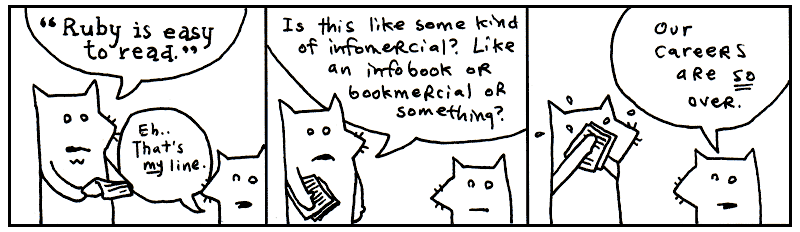
\includegraphics[width=\textwidth]{img/easy_to_read.png}

Lies folgenden Code laut vor:
\lstinputlisting{code/easytoread.rb}

Ruby ist »Coderspeak«, nicht nur eine Programmiersprache. Das obige Programm tut genau das, was erwartet wird, wenn man den Code vorliest.

Ein weiteres Beispiel ist folgender Code:
\lstinputlisting{code/easytoread2.rb}

Der Code beendet das Programm, ausser wenn der String »Restaurant« als Teil »aura« enthält, was auch der Fall ist. Ruby nutzt geschickte \emph{Konventionen}, was die Methodennamen angeht um die Lesbarkeit des Codes zu verbessern. Eine Methode, die am Ende des Names ein Fragezeichen hat, ist eine Ja/Nein-Frage an das Objekt auf dem sie aufgerufen wird (also eine Methode die einen \texttt{boolean} als Rückgabewert hat).

Das soll nicht heissen, dass Code der in einer anderen Sprache geschrieben ist schwer zu lesen ist. Vielfach ist das allerdings so und die Konventionen in Ruby machen viele Teile des Codes einfacher zu lesen und befreien ihn von Überraschungen. Mehr dazu im Kapitel \ref{cha:die_syntax_von_ruby}.


% subsection ruby_ist_einfach_zu_lesen (end)

\subsection*{Alles ist ein Objekt} % (fold)
\label{sub:alles_ist_ein_objekt}
In Ruby ist alles ein Objekt. Wirklich alles --- es gibt in Ruby keine Unterscheidung zwischen »primitiven Datentypen« und »benutzerdefinierten Typen«.
Nachfolgend ein paar Beispiele von Methoden, die auf Instanzen von Klassen aufgerufen werden. Nachgestellt als Kommentar ist jeweils das Resultat eines Statements.
\lstinputlisting{code/objects.rb}
% subsection alles_ist_ein_objekt (end)
% section was_macht_ruby_speziell (end)

\section{Woher kommt Ruby und was ist das Ziel} % (fold)
\label{sec:woher_kommt_ruby_und_was_ist_das_ziel}
Ruby wurde von Yukihiro »Matz« Matsumoto in Japan im Jahre 1995 zum ersten Mal released. Weltweit erreichte die Sprache danach den Ruf einer einfach zu erlernenden, mächtigen und expressiven Sprache.
Die Intention war damals ein »Perl, better than Perl« als Sprache zu entwerfen.

Folgende Kernpunkte sollten Ruby auszeichnen:
\begin{itemize}
	\item Pure OO-Sprache
	\item Simpel und frei von Überraschungen
	\item Mächtige und flexible Sprache
	\item Produktiv: Schnelle Entwicklung
	\item Nicht kommerziell: Ruby ist Open-Source
	\item Robust: Ruby hat einen Garbage-Collector
	\item Flexibel: Dynamisch typisierte Sprache
\end{itemize}

% section woher_kommt_ruby_und_was_ist_das_ziel (end)

% chapter ruby_noch_eine_sprache_ (end)




\chapter{Die Syntax von Ruby} % (fold)
\label{cha:die_syntax_von_ruby}

% chapter die_syntax_von_ruby (end)


\chapter*{Quellen} % (fold)
\label{cha:quellen}
Folgende Quellen lieferten Material für diese Lecture Notes:

\begin{itemize}
	\item »Why's (poignant) guide to ruby«\footnote{\url{http://poignantguide.net/ruby/}}: auflockernde Comics mit den Two Foxes.
\end{itemize}
% chapter quellen (end)

%\bibliography{FungiLit}                                                                                                                                                %\bibliographystyle{plain}                                                                                                                                                     %                         \nocite{*}%
%


\end{document}
